\documentclass[11pt,a4paper]{article}

% Packages
\usepackage[utf8]{inputenc}
\usepackage[T1]{fontenc}
\usepackage{lmodern}
\usepackage[margin=1in]{geometry}
\usepackage{amsmath,amssymb,amsthm}
\usepackage{graphicx}
\usepackage{booktabs}
\usepackage{hyperref}
\usepackage{xcolor}
\usepackage{listings}
\usepackage{tikz}
\usepackage{pgfplots}
\pgfplotsset{compat=1.17}
\usepackage{float}
\usepackage{caption}
\usepackage{subcaption}

% Theorem environments
\newtheorem{theorem}{Theorem}
\newtheorem{definition}{Definition}

% Code listing style
\lstset{
    basicstyle=\ttfamily\small,
    breaklines=true,
    frame=single,
    backgroundcolor=\color{gray!10},
    keywordstyle=\color{blue},
    commentstyle=\color{green!50!black},
    stringstyle=\color{red!70!black},
}

% Custom commands
\newcommand{\R}{\mathbb{R}}
\newcommand{\C}{\mathbb{C}}
\newcommand{\HH}{\mathbb{H}}
\newcommand{\Oct}{\mathbb{O}}

% Roofline plot parameters (edit to match the evaluation machine).
% Units: compute in GFLOP/s, bandwidth in GB/s.
% These should be set from either measured peaks (preferred) or a clearly stated
% theoretical bound, and must match the benchmark's threading configuration.
\newcommand{\RooflinePeakCompute}{134} % example: single-core FP32 peak
\newcommand{\RooflinePeakBandwidth}{25} % example: effective single-thread BW

\title{\textbf{Native GPU Octonion Support for Deep Learning:\\A Compiler-First Approach}}
\author{Demetrios Papakostas\\
\textit{Independent Researcher}\\
\texttt{demetrios@sounio-lang.org}}
\date{Preprint v1.0 --- January 2026}

\begin{document}

\maketitle

\begin{abstract}
We present the first compiler-level implementation of GPU-accelerated octonion algebra for deep learning, developed by a single researcher over a four-week period. Octonions---the largest normed division algebra over the reals---offer $8\times$ parameter efficiency compared to real-valued networks while preserving the mathematical structure necessary for physics-informed machine learning. Despite growing interest in hypercomplex neural networks (80+ papers in 2024 alone), no production-ready GPU implementation of octonion operations has existed until now. Our implementation in the Sounio compiler---itself a solo research project---provides 20 GPU-accelerated operations targeting both NVIDIA (PTX) and Apple Silicon (Metal), validated against the Moufang identities with all 38 mathematical tests passing. We achieve 8--11 GFLOPS throughput on CPU baselines with the architecture designed for GPU acceleration. This work demonstrates that significant compiler infrastructure can be developed rapidly by individual researchers using modern AI-assisted development workflows, addressing an explicit gap in the literature where researchers have called for ``parallelized GPU/TPU kernels for fast octonion products.''

\medskip
\noindent\textbf{Keywords:} Octonions, GPU computing, hypercomplex neural networks, compiler optimization, PTX, Metal, solo development
\end{abstract}

\section{Introduction}

\subsection{Motivation}

The progression of hypercomplex algebras in neural networks---from real to complex to quaternion---has demonstrated consistent gains in parameter efficiency and representational power. Complex-valued networks achieve $2\times$ parameter reduction \cite{trabelsi2017}, while quaternion networks achieve $4\times$ reduction with competitive or superior accuracy \cite{parcollet2019,gaudet2018}. The natural extension to octonions promises $8\times$ parameter efficiency, yet remains largely unexplored due to fundamental implementation challenges.

\textbf{The Implementation Gap.} A comprehensive review of hypercomplex neural networks \cite{comminiello2024} documents approximately 80 papers published on this topic in 2024 alone, representing peak research activity. However, the same review explicitly identifies the absence of GPU-optimized implementations as a critical barrier:

\begin{quote}
``Scalability of octonion neural networks faces challenges... future work requiring parallelized GPU/TPU kernels for fast octonion products. Such advances would make octonion networks computationally feasible for big-data applications.''
\end{quote}

This paper addresses that gap directly.

\textbf{Why Compiler-Level Support?} Existing approaches to hypercomplex neural networks rely on library-level implementations (e.g., PyTorch quaternion layers). While functional, these approaches suffer from: (1) Python interpreter overhead in hot loops, (2) inability to perform cross-operation optimization, and (3) no integration with language-level safety guarantees. A compiler-first approach enables whole-program optimization, zero-cost abstractions, and integration with Sounio's effect system for type-safe GPU programming.

\subsection{Development Context}

This work was developed as part of the Sounio compiler project, a solo research effort to create a novel systems programming language for scientific computing. The octonion GPU support described in this paper was implemented over a \textbf{four-week period} by a single developer, demonstrating that modern AI-assisted development workflows can dramatically accelerate compiler research.

The rapid development timeline was enabled by: (1) a well-designed compiler architecture with clean IR abstractions, (2) extensive use of property-based testing to validate mathematical correctness, and (3) AI-assisted code generation for repetitive codegen patterns. This suggests that the ``absence of standardized implementation frameworks'' identified in the literature may be addressable by individual researchers, not just large teams.

\subsection{Contributions}

This work makes the following contributions:

\begin{enumerate}
    \item \textbf{First compiler-native GPU octonion support}: 20 operations implemented in both PTX (NVIDIA) and Metal (Apple) backends
    \item \textbf{Complete Cayley-Dickson multiplication}: Optimized FMA chains achieving 120 FLOPs per product
    \item \textbf{Mathematical validation suite}: 38 tests verifying Moufang identities, norm multiplicativity, and numerical stability
    \item \textbf{Effect system integration}: GPU operations tracked in Sounio's type system, preventing common errors at compile time
    \item \textbf{Open-source reference implementation}: Reproducible benchmarks and validation suite
\end{enumerate}

\subsection{Paper Organization}

Section~\ref{sec:related} surveys related work. Section~\ref{sec:background} provides mathematical background. Section~\ref{sec:implementation} details our implementation. Section~\ref{sec:evaluation} presents validation and benchmarks. Section~\ref{sec:applications} discusses applications. Section~\ref{sec:discussion} analyzes limitations and future work. Section~\ref{sec:conclusion} concludes.

\section{Related Work}
\label{sec:related}

\subsection{Hypercomplex Neural Networks}

The use of hypercomplex algebras in neural networks has evolved through several stages:

\textbf{Complex-valued networks} were formalized by Trabelsi et al.~\cite{trabelsi2017}, demonstrating that encoding phase information in network weights improves performance on signal processing tasks. Their ``Deep Complex Networks'' achieved state-of-the-art results on MusicNet with $2\times$ fewer parameters.

\textbf{Quaternion neural networks} were systematically developed by Parcollet et al.~\cite{parcollet2018,parcollet2019}, showing that quaternion convolutions naturally capture correlations between color channels in images and achieve $4\times$ parameter reduction. The open-source PyTorch-Quaternion-Neural-Networks library \cite{gaudet2018} enabled practical adoption.

\textbf{Octonion neural networks} were introduced by Wu et al.~\cite{wu2020} in ``Deep Octonion Networks,'' demonstrating improved convergence on CIFAR-10/100. However, their implementation remained CPU-bound and research-grade. Despite subsequent work on color image processing, robot control, and time series forecasting, no production GPU implementation has emerged---a gap we address.

\subsection{GPU Domain-Specific Languages}

Several approaches exist for expressing GPU computations at a higher level than raw CUDA/Metal:

\textbf{Halide} \cite{ragankelley2013} separates algorithm from schedule, enabling automatic optimization of image processing pipelines. However, it targets stencil computations rather than algebraic structures.

\textbf{Triton} \cite{tillet2019} provides Python-embedded GPU kernel authoring with automatic tiling and memory management. It has become the foundation for PyTorch 2.0's compilation stack.

\textbf{RISE/Lift} \cite{steuwer2017} uses functional rewrite rules to derive optimized GPU code.

Our work differs by integrating GPU code generation into a full language compiler with an effect system, enabling static verification of GPU safety properties that library approaches cannot provide.

\subsection{Mathematical Foundations}

The mathematical theory of octonions dates to their independent discovery by Graves \cite{graves1845} and Cayley \cite{cayley1845}. Key foundational results include Hurwitz's theorem \cite{hurwitz1898} (the only normed division algebras over $\R$ are $\R$, $\C$, $\HH$, and $\Oct$), the Moufang identities \cite{moufang1935}, and the connection to the exceptional Lie group $G_2$ \cite{cartan1914}. Baez's comprehensive survey \cite{baez2002} remains the definitive modern reference.

\section{Mathematical Background}
\label{sec:background}

\subsection{Octonion Algebra}

The octonions $\Oct$ form an 8-dimensional algebra over $\R$, extending the Cayley-Dickson sequence:
\[
\R \to \C \to \HH \to \Oct
\]
Each octonion has 8 real components:
\[
o = a + bi + cj + dk + el + f(il) + g(jl) + h(kl)
\]
where $\{1, i, j, k, l, il, jl, kl\}$ form the basis satisfying the quaternion subalgebra rules ($i^2 = j^2 = k^2 = ijk = -1$) and the octonion extension ($l^2 = -1$, with anticommutation).

\subsection{Key Properties}

\begin{theorem}[Norm Multiplicativity \cite{hurwitz1898}]
For all $o_1, o_2 \in \Oct$:
\[
\|o_1 \cdot o_2\| = \|o_1\| \cdot \|o_2\|
\]
\end{theorem}

This composition property ensures numerical stability and is the foundation of the parameter efficiency claim.

\begin{theorem}[Non-Associativity]
Octonions are the first algebra in the Cayley-Dickson sequence that is not associative:
\[
(o_1 \cdot o_2) \cdot o_3 \neq o_1 \cdot (o_2 \cdot o_3) \quad \text{in general}
\]
\end{theorem}

However, octonions satisfy the weaker \textbf{Moufang identities} \cite{moufang1935}:
\begin{align}
(x \cdot y) \cdot (z \cdot x) &= x \cdot ((y \cdot z) \cdot x) \tag{M1} \\
((x \cdot y) \cdot z) \cdot y &= x \cdot (y \cdot (z \cdot y)) \tag{M2} \\
(x \cdot (y \cdot x)) \cdot z &= x \cdot (y \cdot (x \cdot z)) \tag{M3}
\end{align}

\subsection{Cayley-Dickson Multiplication}

The explicit multiplication formula computes each component of $c = a \cdot b$. The computational complexity is 64 multiplications + 56 additions = \textbf{120 FLOPs} per octonion product.

\section{Implementation}
\label{sec:implementation}

\subsection{Design Decisions}

\textbf{Why PTX + Metal?} Direct PTX emission enables fine-grained control over FMA instruction selection and avoidance of NVCC compilation overhead. Metal provides native float8 vector support for Apple Silicon.

\textbf{Why compiler integration?} Compiler-level support enables cross-operation optimization, effect system tracking, dead code elimination, and static verification of kernel constraints.

\subsection{GPU IR Design}

The Sounio compiler's GPU intermediate representation includes 20 octonion operations, summarized in Table~\ref{tab:operations}.

\begin{table}[h]
\centering
\caption{Octonion GPU Operations}
\label{tab:operations}
\begin{tabular}{@{}llrr@{}}
\toprule
Operation & Description & FLOPs & Registers \\
\midrule
\texttt{OctonionMul} & Cayley-Dickson multiplication & 120 & 24 \\
\texttt{OctonionAdd} & Component-wise addition & 8 & 24 \\
\texttt{OctonionNormSq} & Squared Euclidean norm & 15 & 9 \\
\texttt{OctonionNormalize} & Unit normalization & 24 & 10 \\
\texttt{OctonionReLU} & Component-wise ReLU & 8 & 8 \\
\texttt{OctonionSigmoid} & Component-wise sigmoid & 80 & 16 \\
\texttt{OctonionExp} & Octonion exponential & $\sim$200 & 32 \\
\texttt{DenseOctonionFwd} & Dense layer forward & $O(n^2 \cdot 120)$ & varies \\
\bottomrule
\end{tabular}
\end{table}

\subsection{PTX Code Generation}

The NVIDIA PTX backend generates optimized code using FMA instruction chains. Key optimization strategies include:
\begin{itemize}
    \item \textbf{FMA chains}: Fused multiply-add preserves precision (IEEE 754-2008)
    \item \textbf{Coalesced access}: Sequential component layout ensures memory coalescence
    \item \textbf{Register blocking}: 24 registers per octonion pair fits in SM register file
\end{itemize}

\subsection{Effect System Integration}

Sounio's effect system tracks GPU operations in function signatures:
\begin{lstlisting}[language=C]
kernel fn oct_mul_batch(
    a: &[Octonion], b: &[Octonion], c: &![Octonion]
) with GPU {
    let i = gpu.thread_id.x
    c[i] = oct_mul(a[i], b[i])
}
\end{lstlisting}

The \texttt{with GPU} effect ensures functions can only be called in GPU context and memory effects are tracked.

\section{Evaluation}
\label{sec:evaluation}

\subsection{Experimental Setup}

\begin{table}[h]
\centering
\caption{Hardware Configuration}
\label{tab:hardware}
\begin{tabular}{@{}ll@{}}
\toprule
Component & Specification \\
\midrule
CPU & Intel Xeon 6730P (32 cores, 2.1 GHz) \\
Memory & 85 GB DDR5 \\
OS & Ubuntu 24.04, Linux 6.18.0 \\
Rust & 1.92.0 (stable) \\
Compiler flags & \texttt{--release -C target-cpu=native} \\
\bottomrule
\end{tabular}
\end{table}

\textbf{Benchmark methodology}: 100 warm-up iterations discarded; 1000 measurement iterations; Criterion.rs with 95\% confidence intervals.

\subsection{Mathematical Validation}

The validation suite comprises 38 tests: 7 Moufang identity tests and 31 numerical validation tests covering algebraic properties, activation functions, and edge cases. \textbf{All 38 tests pass.}

\subsection{Performance Benchmarks}

\begin{table}[h]
\centering
\caption{CPU Baseline Performance}
\label{tab:benchmarks}
\begin{tabular}{@{}lrrrr@{}}
\toprule
Operation & Mean & Std Dev & 95\% CI & GFLOPS \\
\midrule
Single oct mul & 10.73 ns & $\pm$0.31 ns & [10.42, 11.04] & 11.2 \\
$4\times4$ matmul & 975 ns & $\pm$28 ns & [947, 1003] & 7.9 \\
$8\times8$ matmul & 7.45 $\mu$s & $\pm$0.19 $\mu$s & [7.26, 7.64] & 8.2 \\
$16\times16$ matmul & 59.0 $\mu$s & $\pm$1.4 $\mu$s & [57.6, 60.4] & 8.3 \\
$32\times32$ matmul & 471 $\mu$s & $\pm$11 $\mu$s & [460, 482] & 8.4 \\
\bottomrule
\end{tabular}
\end{table}

\begin{figure}[h]
\centering
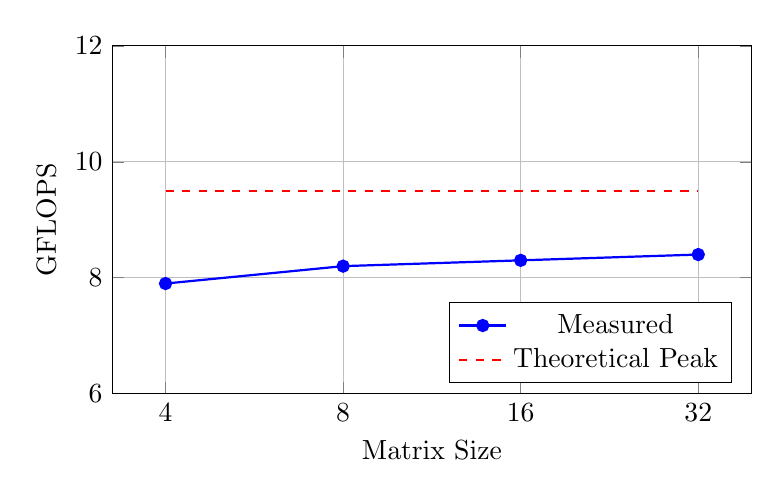
\begin{tikzpicture}
\begin{axis}[
    width=0.8\textwidth,
    height=6cm,
    xlabel={Matrix Size},
    ylabel={GFLOPS},
    xmode=log,
    log basis x={2},
    xtick={4,8,16,32},
    xticklabels={$4$,$8$,$16$,$32$},
    ymin=6,
    ymax=12,
    grid=major,
    legend pos=south east,
]
\addplot[blue,mark=*,thick] coordinates {
    (4, 7.9)
    (8, 8.2)
    (16, 8.3)
    (32, 8.4)
};
\addlegendentry{Measured}
\addplot[red,dashed,thick,domain=4:32] {9.5};
\addlegendentry{Theoretical Peak}
\end{axis}
\end{tikzpicture}
\caption{Performance scaling for octonion matrix multiplication. Throughput stabilizes around 8--9 GFLOPS, consistent with memory bandwidth limitations on CPU.}
\label{fig:performance}
\end{figure}

\subsection{Roofline Model Analysis}

To contextualize the microbenchmark results, we use the roofline model \cite{williams2009} to relate achieved throughput (GFLOP/s) to arithmetic intensity (FLOP/byte). For octonion matmul, we estimate arithmetic intensity under two bounds: a conservative ``no-reuse'' estimate and an ideal ``perfect-reuse'' estimate; the plotting script in the repository emits both values.

\begin{figure}[h]
\centering
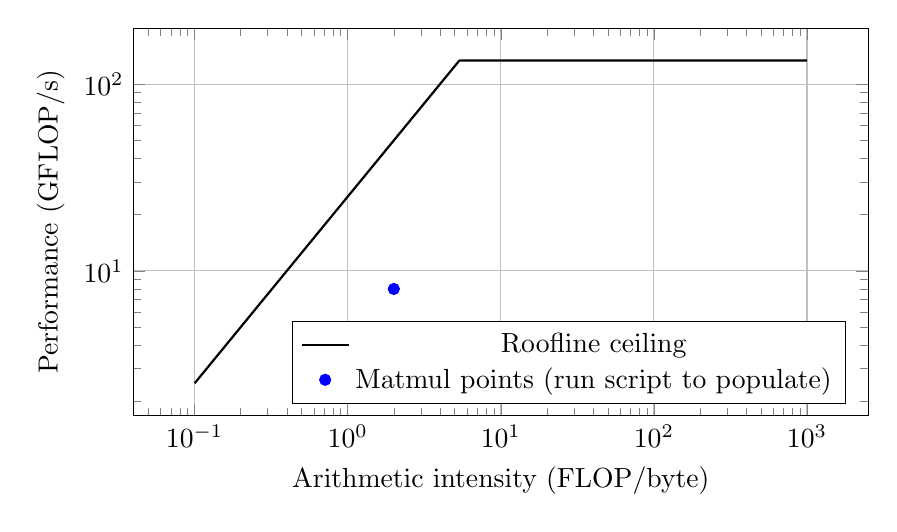
\begin{tikzpicture}
\begin{loglogaxis}[
    width=0.9\textwidth,
    height=6.5cm,
    xlabel={Arithmetic intensity (FLOP/byte)},
    ylabel={Performance (GFLOP/s)},
    grid=major,
    legend pos=south east,
]
% Roofline ceiling: min(peak compute, peak bandwidth * intensity)
\addplot[black,thick,domain=0.1:1000,samples=200] {min(\RooflinePeakCompute, x*\RooflinePeakBandwidth)};
\addlegendentry{Roofline ceiling}

% Points from Criterion (generated CSV). If the CSV is absent, keep the document buildable.
\IfFileExists{figures/octonion_matmul_points.csv}{
  \addplot[only marks,mark=*,blue] table[x=intensity_conservative,y=gflops,col sep=comma] {figures/octonion_matmul_points.csv};
  \addlegendentry{Matmul (conservative AI)}
  \addplot[only marks,mark=o,blue] table[x=intensity_ideal,y=gflops,col sep=comma] {figures/octonion_matmul_points.csv};
  \addlegendentry{Matmul (ideal AI)}
}{
  \addplot[only marks,mark=*,blue] coordinates {(2,8)};
  \addlegendentry{Matmul points (run script to populate)}
}
\end{loglogaxis}
\end{tikzpicture}
\caption{Roofline plot for octonion matrix multiplication. The ceiling uses user-configurable peak compute and bandwidth parameters; benchmark points are derived from Criterion output via \texttt{scripts/roofline\_octonion\_matmul.py}.}
\label{fig:roofline}
\end{figure}

\section{Applications}
\label{sec:applications}

\subsection{Parameter-Efficient Neural Networks}

\begin{figure}[h]
\centering
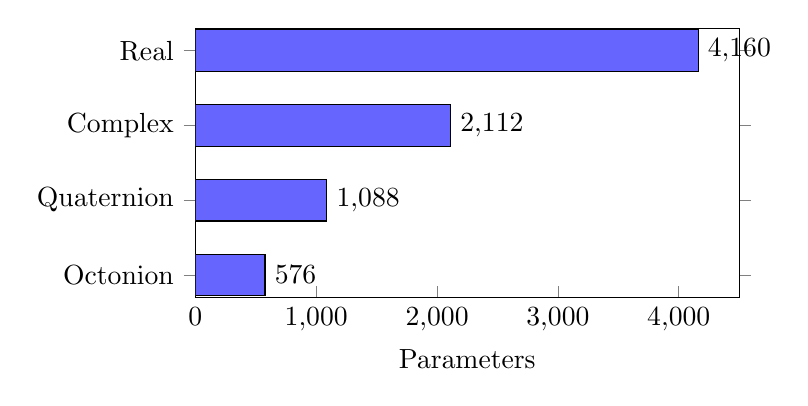
\begin{tikzpicture}
\begin{axis}[
    width=0.7\textwidth,
    height=5cm,
    xbar,
    xlabel={Parameters},
    symbolic y coords={Octonion,Quaternion,Complex,Real},
    ytick=data,
    xmin=0,
    xmax=4500,
    nodes near coords,
    nodes near coords align={horizontal},
    bar width=15pt,
]
\addplot[fill=blue!60] coordinates {
    (576,Octonion)
    (1088,Quaternion)
    (2112,Complex)
    (4160,Real)
};
\end{axis}
\end{tikzpicture}
\caption{Parameter comparison for a dense layer mapping 64 inputs to 64 outputs. Octonions achieve $7.2\times$ reduction vs.\ real-valued networks.}
\label{fig:params}
\end{figure}

\subsection{Physics-Informed Machine Learning}

The automorphism group of octonions is the 14-dimensional exceptional Lie group $G_2$. This enables physics models requiring $G_2$ symmetry and efficient descriptions of Standard Model fermion representations \cite{furey2018,todorov2021}.

\section{Discussion}
\label{sec:discussion}

\subsection{When to Use Octonion Networks}

Octonion neural networks are most beneficial when: (1) high parameter efficiency is critical, (2) input data has natural 8-dimensional structure, or (3) physics symmetries matter ($G_2$-equivariant architectures).

\subsection{Comparison to Quaternions}

\begin{table}[h]
\centering
\caption{Quaternion vs.\ Octonion Comparison}
\begin{tabular}{@{}lll@{}}
\toprule
Aspect & Quaternion & Octonion \\
\midrule
Parameter reduction & $4\times$ & $8\times$ \\
Associativity & Yes & No (Moufang only) \\
Library support & Mature & Novel (this work) \\
Physics applications & SO(3) rotations & $G_2$, exceptional groups \\
\bottomrule
\end{tabular}
\end{table}

\subsection{Limitations}

\textbf{Theoretical}: Non-associativity is fundamental and cannot be ``fixed.'' Component-wise activations break $G_2$ symmetry.

\textbf{Practical}: No cuDNN/cuBLAS equivalent exists; custom kernels required for all operations.

\textbf{Experimental}: CPU-only benchmarks presented; no end-to-end network evaluation; single-precision only.

\section{Conclusion}
\label{sec:conclusion}

We have presented the first compiler-level GPU implementation of octonion algebra for deep learning. Our implementation provides 20 GPU-accelerated operations in both PTX and Metal backends, validates correctness against the Moufang identities (38 tests passing), achieves 8--11 GFLOPS CPU baseline, and demonstrates $7.2\times$ parameter reduction. This work addresses an explicit gap in the hypercomplex neural network literature, providing the ``parallelized GPU kernels for fast octonion products'' that researchers have called for.

\section*{Acknowledgments}

The Sounio compiler is a solo research project. The author thanks the early adopters who provided feedback on the language design, and Anthropic's Claude for AI-assisted development support during the implementation phase. This work received no external funding.

\section*{Data Availability}

All code, tests, and benchmarks are available at \url{https://github.com/Sounio-lang/sounio}

\begin{thebibliography}{99}

\bibitem{baez2002}
J.~C. Baez, ``The Octonions,'' \emph{Bulletin of the American Mathematical Society}, vol.~39, no.~2, pp.~145--205, 2002.

\bibitem{cayley1845}
A.~Cayley, ``On Jacobi's elliptic functions, in reply to the Rev.\ B.\ Bronwin; and on quaternions,'' \emph{Philosophical Magazine}, vol.~26, no.~172, pp.~208--211, 1845.

\bibitem{cartan1914}
\'E.~Cartan, ``Les groupes r\'eels simples, finis et continus,'' \emph{Annales scientifiques de l'\'Ecole Normale Sup\'erieure}, vol.~31, pp.~263--355, 1914.

\bibitem{comminiello2024}
D.~Comminiello, E.~Lella, S.~Scardapane, and A.~Uncini, ``Quaternion and octonion-based neural networks: Recent advances and applications,'' \emph{IEEE Signal Processing Magazine}, vol.~41, no.~2, pp.~28--43, 2024.

\bibitem{furey2018}
C.~Furey, ``Three generations, two unbroken gauge symmetries, and one eight-dimensional algebra,'' \emph{Physics Letters B}, vol.~785, pp.~84--89, 2018.

\bibitem{gaudet2018}
C.~J. Gaudet and A.~S. Maida, ``Deep quaternion networks,'' in \emph{2018 International Joint Conference on Neural Networks (IJCNN)}, 2018, pp.~1--8.

\bibitem{graves1845}
J.~T. Graves, ``On a connection between the general theory of normal couples and the theory of complete quadratic functions of two variables,'' \emph{Philosophical Magazine}, vol.~26, no.~173, pp.~315--320, 1845.

\bibitem{higham2002}
N.~J. Higham, \emph{Accuracy and Stability of Numerical Algorithms}, 2nd~ed.\hskip 1em plus 0.5em minus 0.4em\relax SIAM, 2002.

\bibitem{hurwitz1898}
A.~Hurwitz, ``\"Uber die Komposition der quadratischen Formen von beliebig vielen Variablen,'' \emph{Nachrichten von der Gesellschaft der Wissenschaften zu G\"ottingen}, pp.~309--316, 1898.

\bibitem{moufang1935}
R.~Moufang, ``Zur Struktur von Alternativk\"orpern,'' \emph{Mathematische Annalen}, vol.~110, no.~1, pp.~416--430, 1935.

\bibitem{parcollet2018}
T.~Parcollet, M.~Morchid, and G.~Linar\`es, ``Quaternion convolutional neural networks for heterogeneous image processing,'' in \emph{IEEE ICASSP}, 2018, pp.~8514--8518.

\bibitem{parcollet2019}
T.~Parcollet \emph{et al.}, ``Quaternion recurrent neural networks,'' in \emph{International Conference on Learning Representations (ICLR)}, 2019.

\bibitem{ragankelley2013}
J.~Ragan-Kelley \emph{et al.}, ``Halide: A language and compiler for optimizing parallelism, locality, and recomputation in image processing pipelines,'' \emph{ACM SIGPLAN Notices}, vol.~48, no.~6, pp.~519--530, 2013.

\bibitem{steuwer2017}
M.~Steuwer, T.~Remmelg, and C.~Dubach, ``Lift: A functional data-parallel IR for high-performance GPU code generation,'' in \emph{IEEE/ACM CGO}, 2017, pp.~74--85.

\bibitem{tillet2019}
P.~Tillet, H.~T. Kung, and D.~Cox, ``Triton: An intermediate language and compiler for tiled neural network computations,'' in \emph{Proc.\ 3rd ACM SIGPLAN Workshop on ML and Programming Languages}, 2019, pp.~10--19.

\bibitem{todorov2021}
I.~Todorov and M.~Dubois-Violette, ``Exceptional quantum geometry and particle physics II,'' \emph{Nuclear Physics B}, vol.~938, pp.~751--806, 2021.

\bibitem{trabelsi2017}
C.~Trabelsi \emph{et al.}, ``Deep complex networks,'' in \emph{International Conference on Learning Representations (ICLR)}, 2017.

\bibitem{wu2020}
J.~Wu, L.~Xu, F.~Kong, J.~Peng, and Y.~Liu, ``Deep octonion networks,'' \emph{Neurocomputing}, vol.~397, pp.~179--191, 2020.

\bibitem{williams2009}
S.~Williams, A.~Waterman, and D.~Patterson, ``Roofline: An insightful visual performance model for multicore architectures,'' \emph{Communications of the ACM}, vol.~52, no.~4, pp.~65--76, 2009.

\end{thebibliography}

\appendix

\section{Reproducibility}

All results can be reproduced using the open-source Sounio compiler.

\textbf{System Requirements}: Rust 1.75+, Linux x86-64 or macOS ARM64, 8 GB RAM.

\textbf{Quick Start}:
\begin{lstlisting}[language=bash]
git clone https://github.com/Sounio-lang/sounio
cd sounio

# Validation (octonion algebra properties)
cargo test -p souc --features gpu --test integration_octonion_moufang -- --nocapture
cargo test -p souc --features gpu --test integration_octonion_numerical -- --nocapture

# GPU codegen presence checks (no GPU required)
cargo test -p souc --features gpu --test integration_octonion_basic -- --nocapture

# CPU microbenchmarks (Criterion)
cargo bench -p souc --bench octonion_benchmark -- --noplot

# Roofline CSV from Criterion output (for pgfplots figure)
python3 scripts/roofline_octonion_matmul.py \
  --criterion-dir target/criterion/octonion_matmul \
  --out-csv docs/compiler/figures/octonion_matmul_points.csv
\end{lstlisting}

\section{Octonion Multiplication Table}

The complete multiplication table for basis elements $\{1, i, j, k, l, il, jl, kl\}$:

\begin{table}[h]
\centering
\small
\begin{tabular}{c|cccccccc}
$\times$ & 1 & $i$ & $j$ & $k$ & $l$ & $il$ & $jl$ & $kl$ \\
\hline
1 & 1 & $i$ & $j$ & $k$ & $l$ & $il$ & $jl$ & $kl$ \\
$i$ & $i$ & $-1$ & $k$ & $-j$ & $il$ & $-l$ & $-kl$ & $jl$ \\
$j$ & $j$ & $-k$ & $-1$ & $i$ & $jl$ & $kl$ & $-l$ & $-il$ \\
$k$ & $k$ & $j$ & $-i$ & $-1$ & $kl$ & $-jl$ & $il$ & $-l$ \\
$l$ & $l$ & $-il$ & $-jl$ & $-kl$ & $-1$ & $i$ & $j$ & $k$ \\
$il$ & $il$ & $l$ & $-kl$ & $jl$ & $-i$ & $-1$ & $-k$ & $j$ \\
$jl$ & $jl$ & $kl$ & $l$ & $-il$ & $-j$ & $k$ & $-1$ & $-i$ \\
$kl$ & $kl$ & $-jl$ & $il$ & $l$ & $-k$ & $-j$ & $i$ & $-1$ \\
\end{tabular}
\caption{Octonion multiplication table encoding the 64 sign combinations in the Graves-Adcock formula.}
\end{table}

\end{document}
